\documentclass{./civarticle}
\usepackage{graphicx} % Required for inserting images

\title{Эссе по теме "Криптографические хеш-функции"}
\author{Костиков Егор Вячеславович}
\date{Апрель 2024}

\begin{document}

\maketitle

\section{Введение}

В данной работе приводится описание основных архитектур, используемых при построении современных хеш-функций (Sponge-конструкция, конструкция HAIFA), а также приводятся описания реализации следующих хеш-функций: MD5, SHA-1, SHA-256, SHA-3, ГОСТ Р 34.11-94, ГОСТ 34.11-2018 (Стрибог), BLAKE-256, RIPEMD-256, Whirlpool, Fast Syndrome Based Hash (FSB). Также приводится более подробное описание и анализ хеш-функции RIPEMD-256 (на основе известных результатов анализа RIPEMD-128).

\section{Термины и определения}

Криптографической функцией хеширования (хеш-функцией) называется отображение $H: V^{*} \rightarrow V_n$, где $n$ --- натуральное число, $V^{*}$ --- множество всех двоичных векторов конечной размерности (включая пустую строку), $V_n$ --- множество всех $n$-мерных двоичных векторов. Возвращаемое хеш-функцией значение называется хеш-значением.

Коллизионная атака на хеш-функцию --- поиск двух различных входных блоков криптографической хеш-функции, производящих одинаковые значения хеш-функции.

Далее в работе используются следующие обозначения:
\begin{itemize}
    \item $X <<< n$ --- циклический сдвиг содержимого $X$ на $n$ бит влево;
    \item $X >>> n$ --- циклический сдвиг содержимого $X$ на $n$ бит вправо;
    \item $X << n$ --- сдвиг содержимого $X$ на $n$ бит влево (с дописыванием нулевого бита);
    \item $X >> n$ --- сдвиг содержимого $X$ на $n$ бит вправо (с дописыванием нулевого бита);
    \item $x \mathbin\Vert y$ --- конкатенация строк $x$ и $y$;
    \item $x \oplus y$ --- побитовое сложение $x$ и $y$;
    \item $GF(q)$ --- конечное поле Галуа, содержащее $q$ элементов.
\end{itemize}

\section{Описание архитектур хеш-функций}

\subsection{Sponge-конструкция}

Конструкция Sponge была впервые представлена в 2007 году в работе \cite{sponge}. 

"Губка" состоит из внутреннего состояния $S$, содержащее данные фиксированного размера в $b$ бит. Состояние разбивается на две части: первая часть имеет размер $r$, вторая --- $c$ ($b = r + c$). Изначально все биты состояния инициализируются нулями. Входное сообщение $M$ дополняется некоторой функцией $pad$, после выполнения которой длина дополненного сообщения становится кратна заданной длине блока сообщения, и разбивается на $r$-битовые блоки. Также в работе "губки" участвует внутренняя $b$-битная функция $f$. Работа "губки" состоит из двух фаз:

\begin{itemize}
    \item Фаза "впитывания" (absorbing phase)

    На данном этапе $r$-битные блоки исходного сообщения $M$ подвергаются операции побитового сложения с первой частью состояния, результат сохраняется в $r$-битовой части состояния, после чего все обновленное состояние поступает на вход функции $f$. Когда все блоки сообщения обработаны подобным образом, то "губка" переходит в фазу "выжимания".

    \item Фаза "выжимания" (squeezing phase)

    На данном этапе первая часть состояния возвращается в качестве выходных блоков, после чего все состояние поступает на вход функции $f$. Количество операций определяется запрошенным количеством бит $l$.
    
\end{itemize}

После последней итерации вывод обрезается до первых $l$ бит.

\begin{figure}[h!]
        \center{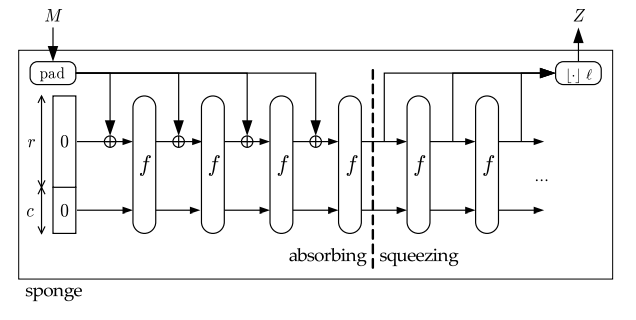
\includegraphics[width=0.7\linewidth]{sponge.png} \\ Конструкция sponge \cite{sponge2}}
        \end{figure}

Стоит отметить, что хеш-функции, построенные на основе конструкции sponge могут быть отличены от случайного оракула только за счет внутренних коллизий, что свидетельствует о высокой степени сходства с идеальным случайным оракулом и обеспечивает надежность и безопасность применения sponge-функций.


\subsection{Конструкция HAIFA}

Конструкция HAIFA (The HAsh Iterative FrAmework) была впервые предложена в 2007 году в работе \cite{haifa}. Конструкция HAIFA заменяет традиционную конструкцию Меркла-Дамгарда. HAIFA улучшает безопасность хеш-функций, поддерживает определение семейств хеш-функций и переменный размер хеш-значения.

Стандартная конструкция Меркла-Дамгарда заключается в следующем:

\begin{itemize}
    \item Пусть на вход поступило сообщение $M$, разбитое на $k$ $n$-битовых блоков $M = M_1 \mathbin\Vert ... \mathbin\Vert M_k$; пусть также определено некоторое значение $m_c$-битного вектора инициализации $h_0 = IV$.
    \item Пусть определена функция сжатия $C = C(h, M)$, принимающая $m_c$-битное значение $h$ и $n$-битное значение $M$.
    \item Далее $k$ раз производятся обращения к функции сжатия: $h_i = C(h_{i-1}, M_i)$, $i = 1, ..., k$;
    \item Полученное на $k$-ой итерации значение $h_k$ возвращается в качестве хеш-значения сообщения $M$.
\end{itemize}

В конструкции HAIFA функция сжатия имеет следующий вид: $C = C(h, M, bits, salt)$, где $h$ --- $m_c$-битный блок, $M$ --- $n$-битный блок, $bits$ --- количество бит, захешированных к этому времени, $salt$ --- используемая соль.

В HAIFA обязательным шагом при хешировании является расширение сообщения: при этом используется следующая схема расширения:

\begin{enumerate}
    \item Сообщение дополняется одним единичным битом;
    \item Сообщение дополняется необходимым числом нулевых битов, чтобы длина дополняемого сообщения стала сравнима по модулю $n$ с $n - (t + r)$.
    \item Сообщение расширяется за счет приписывания $t$-битового значения длины сообщения;
    \item Сообщение расширяется за счет приписывания $r$-битового значения хешированного блока.
\end{enumerate}

В HAIFA реализована возможность изменять размер хеша. Пусть $IV$ --- начальное значение, выбранное разработчиком функции сжатия, пусть $m$ --- требуемая длина выхода. Для создания хеш-функции из $m$ бит вычисляется следующее начальное значение: $IV_m = C(IV, m, 0, 0)$. В результате получается значение $m$, "закодированное" первыми $r$ битами, за которым идет единичный бит и $n-r-1$ нулевых битов. После того, как посчитался последний блок, итоговым значением являются $m$ бит последнего значения функции сжатия цепочки.

Таким образом, для хеширования сообщения необходимо проделать следующие действия:

\begin{itemize}
    \item Расширить сообщение так, как было описано ранее;
    \item Подсчитать значение $IV_m$ так, как было описано ранее;
    \item В цикле обработать все блоки дополненного сообщения, вычисляя значение функции сжатия:\\ $h_i = C(h_{i-1}, M_i, bits, salt)$;
    \item В случае необходимости обрезать последнее полученное значение до нужного числа бит.
\end{itemize}

Конструкция HAIFA обеспечивает улучшенную стойкость по сравнению с традиционной конструкцией Меркла-Дамгарда. Добавление параметров, таких как количество захешированных бит и значение соли, помогает предотвратить различные виды атак, такие как атаки поиска первого и второго прообраза. Кроме того, HAIFA поддерживает различные режимы итерации для функций сжатия, что позволяет адаптировать хеш-функции под конкретные требования безопасности и производительности.

Одним из недостатков HAIFA является возможность использования предварительных вычислений для обхода безопасности, если длина соли ($salt$) недостаточно велика. Рекомендуется, чтобы длина соли составляла как минимум 64 бита или, по возможности, как минимум $\frac{m_c}{2}$ бит, чтобы предотвратить такие атаки. Также отмечается, что для некоторых атак HAIFA требует более длинную соль, чем другие конструкции, что может оказать плохое влияние на производительность.

\section{Описания хеш-функций}

\subsection{MD5}

Описание алгоритма работы хеш-функции MD5 приводится в соответствии со стандартом \cite{md5}. На вход алгоритма поступает двоичное сообщение $m = m_0m_1 ... m_{b-1}$ длины $b \geq 0$ бит; на выходе алгоритм выдает 128-битный хеш входного сообщения. Опишем шаги алгоритма:
\begin{enumerate}
    \item Расширение сообщения

    Сообщение расширяется путем добавления в конец сообщения битов по следующему правилу:

    \begin{enumerate}
        \item В конец сообщения добавляется один единичный бит;
        \item После этого в конец сообщения добавляются нулевые биты до тех пор, пока длина сообщения не станет сравнима с 448 по модулю 512.
    \end{enumerate}

    \item Добавление длины

    Сообщение дополнительно расширяется путем добавления в конец сообщения 64-битного представления длины сообщения $b$. При этом, если $b > 2^{64}$, то добавляются только младшие 64 бита двоичного представления $b$. Данные биты добавляются как два 32-битных слова, причем сначала добавляются младшие 32 бита, а затем старшие.

    После данных преобразований длина сообщения оказывается кратной 512.

    \item Инициализация буфера

    При вычислении значения хеш-функции используются четыре 32-битных регистра A, B, C и D, которые перед началом работы инициализируются следующими 16-ричными значениями:

    \begin{itemize}
        \item A $= 0x01234567$;
        \item B $= 0x89ABCDEF$;
        \item C $= 0xFEDCBA98$;
        \item D $= 0x76543210$.
    \end{itemize}

    \item Обработка сообщения

    Определим четыре вспомогательных функции $F(X, Y, Z), G(X, Y, Z), H(X, Y, Z), I(X, Y, Z)$, принимающих на вход три 32-битных слова и возвращающих одно 32-битное значение:

    \begin{itemize}
        \item $F(X, Y, Z) = (X \wedge Y) \vee (\bar X \wedge Z)$;
        \item $G(X, Y, Z) = (X \wedge Z) \vee (Y \wedge \bar Z)$;
        \item $H(X, Y, Z) = X \oplus Y \oplus Z$;
        \item $I(X, Y, Z) = Y \oplus (X \vee \bar Z)$.
    \end{itemize}

    Определим вспомогательную таблицу $T = T[1] ... T[64]$, состоящую из 64 элементов, где \\ $T[i] = int|4294967296 \cdot \sin(i)|$, где $int$ --- функция взятия целой части. 

    Обработка исходного сообщения происходит в цикле блоками по 512 бит --- на новой итерации очередной блок помещается во вспомогательный массив $X = X[0] ... X[15]$, состоящий из шестнадцати 32-битных слов. Предварительно сохраняются значения регистров A, B, C и D после предыдущей итерации (или начальные значения для первой итерации): AA = A, BB = B, CC = C, DD = D. Выполняются четыре раунда, в каждом из которых совершаются шестнадцать однотипных операций:

    \begin{itemize}
        \item Первый раунд

        Обозначим через $[abcd$ $k$ $s$ $i]$ следующую операцию: $a = b + ((a + F(b,c,d) + X[k] + T[i]) <<< s)$.

        \begin{figure}[h!]
        \center{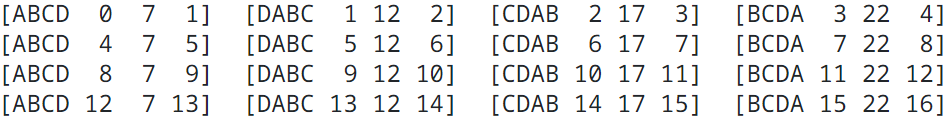
\includegraphics[width=0.7\linewidth]{md5_1.png} \\ Операции первого раунда}
        \end{figure}

        \item Второй раунд

        Обозначим через $[abcd$ $k$ $s$ $i]$ следующую операцию: $a = b + ((a + G(b,c,d) + X[k] + T[i]) <<< s)$.

        \begin{figure}[h!]
        \center{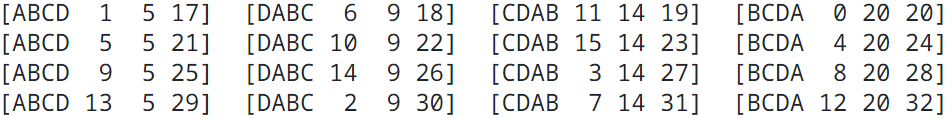
\includegraphics[width=0.7\linewidth]{md5_2.png} \\ Операции второго раунда}
        \end{figure}

        \item Третий раунд

        Обозначим через $[abcd$ $k$ $s$ $i]$ следующую операцию: $a = b + ((a + H(b,c,d) + X[k] + T[i]) <<< s)$.

        \begin{figure}[h!]
        \center{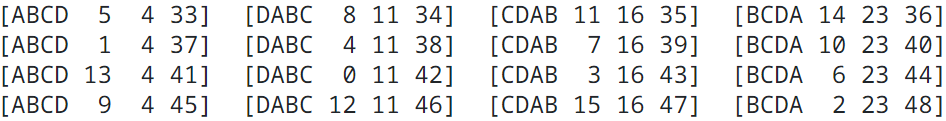
\includegraphics[width=0.7\linewidth]{md5_3.png} \\ Операции третьего раунда}
        \end{figure}

        \item Четвертый раунд

        Обозначим через $[abcd$ $k$ $s$ $i]$ следующую операцию: $a = b + ((a + I(b,c,d) + X[k] + T[i]) <<< s)$.

        \begin{figure}[h!]
        \center{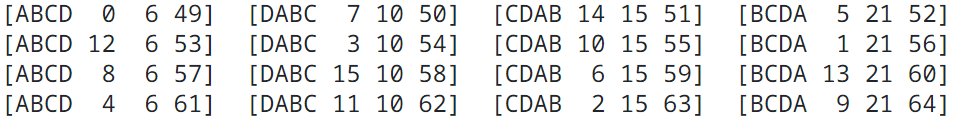
\includegraphics[width=0.7\linewidth]{md5_4.png} \\ Операции четвертого раунда}
        \end{figure}

        \item Действия по окончании итерации: A = AA + A; B = BB + B; C = CC + C; D = DD + D.
        
    \end{itemize}

    \item Результат вычислений

    Результатом вычисления хеш-функции MD5 является 128-битное значение A$\mathbin\Vert$B$\mathbin\Vert$C$\mathbin\Vert$D, составленное из содержимого соответствующих регистров после последней итерации.
    
\end{enumerate}

\subsection{SHA-1}

Описание хеш-функции SHA-1 приводится в соответствии с текстом стандарта \cite{sha1}. На вход алгоритма поступает произвольное двоичное сообщение, состоящее из не более чем $2^{64} - 1$ бит; на выходе алгоритм выдает 160-битное хеш-значение входного сообщения. Опишем алгоритм SHA-1:

\begin{enumerate}
    \item Расширение сообщения

    Сообщение расширяется путем добавления в конец сообщения битов по следующему правилу:

    \begin{enumerate}
        \item В конец сообщения добавляется один единичный бит;
        \item После этого в конец сообщения добавляются нулевые биты до тех пор, пока длина сообщения не станет сравнима с 448 по модулю 512.
    \end{enumerate}

    \item Добавление длины

    Сообщение дополнительно расширяется путем добавления в конец сообщения 64-битного представления длины сообщения. Данные биты добавляются как два 32-битных слова, причем сначала добавляются старшие 32 бита, а затем младшие.

    После данных преобразований длина сообщения оказывается кратной 512.

    \item Инициализация буфера

    При вычислении значения хеш-функции используются пять 32-битных регистра H$_0$, H$_1$, H$_2$, H$_3$ и H$_4$, которые перед началом работы инициализируются следующими 16-ричными значениями:

    \begin{itemize}
        \item H$_0$ $= 0x67452301$;
        \item H$_1$ $= 0xEFCDAB89$;
        \item H$_2$ $= 0x98BADCFE$;
        \item H$_3$ $= 0x10325476$;
        \item H$_4$ $= 0xC3D2E1F0$.
    \end{itemize}

    \item Обработка сообщения

    Определим четыре вспомогательные параметрические функции, принимающие и возвращающие 32-битные значения:

    \begin{itemize}
        \item $f_t(B, C, D) = (B \wedge C) \vee (\bar B \wedge D)$, где $0 \leq t \leq 19$;
        \item $f_t(B, C, D) = B \oplus C \oplus D$, где $20 \leq t \leq 39$;
        \item $f_t(B, C, D) = (B \wedge C) \vee (B \wedge D) \vee (C \wedge D)$, где $40 \leq t \leq 59$;
        \item $f_t(B, C, D) = B \oplus C \oplus D$, где $60 \leq t \leq 79$.
    \end{itemize}

    Также определим следующие константы:
    \begin{itemize}
        \item $K_t = 0x5A827999$, где $0 \leq t \leq 19$;
        \item $K_t = 0x6ED9EBA1$, где $20 \leq t \leq 39$;
        \item $K_t = 0x8F1BBCDC$, где $40 \leq t \leq 59$;
        \item $K_t = 0xCA62C1D6$, где $60 \leq t \leq 79$.
    \end{itemize}

    Обработка исходного сообщения происходит в цикле блоками по 512 бит --- на новой итерации очередной блок помещается во вспомогательный массив $W = W[0] ... W[15]$, состоящий из шестнадцати 32-битных слов. Очередная итерация состоит из следующих действий:

    \begin{enumerate}
        \item $W[t] = (W[t-3] \oplus W[t-8] \oplus W[t-14] \oplus W[t-16]) <<< 1$, для $16 \leq t \leq 79$;
        \item Сохраняются значения вспомогательных регистров: $A$ = H$_0$; $B$ = H$_1$; $C$ = H$_2$; $D$ = H$_3$; $E$ = H$_4$.
        \item $For$ $t$ $=$ $0$ $to$ $79$ $do$ \{ 

        \hspace{0.5cm} $TEMP$ = $A <<< 5 + f_t(B, C, D) + E + W[t] + K_t$;

        \hspace{0.5cm} $E = D; D = C; C = B <<< 30; B = A; A = TEMP$;
    
        \}
        \item Действия по окончании итерации: H$_0$ = H$_0 + A$; H$_1$ = H$_1 + B$; H$_2$ = H$_2 + C$; H$_3$ = H$_3 + D$; H$_4$ = H$_4 + E$.  
    \end{enumerate}

    \item Результат вычислений

    Результатом вычисления хеш-функции SHA-1 является 160-битное значение H$_0\mathbin\Vert$H$_1\mathbin\Vert$H$_2\mathbin\Vert$H$_3\mathbin\Vert$H$_4$, составленное из содержимого соответствующих регистров после последней итерации.
    
\end{enumerate}

\subsection{SHA-256}

Описание алгоритма SHA-256 приводится в соответствии с описанием, приведенным в стандарте \cite{sha256}. На вход алгоритма поступает произвольное двоичное сообщение, состоящее из не более чем $2^{64} - 1$ бит; на выходе алгоритм выдает 256-битный хеш входного сообщения. Опишем шаги данного алгоритма:

\begin{enumerate}
    \item Расширение сообщения

    Сообщение расширяется путем добавления в конец сообщения битов по следующему правилу:

    \begin{enumerate}
        \item В конец сообщения добавляется один единичный бит;
        \item После этого в конец сообщения добавляются нулевые биты до тех пор, пока длина сообщения не станет сравнима с 448 по модулю 512.
    \end{enumerate}

    \item Добавление длины

    Сообщение дополнительно расширяется путем добавления в конец сообщения 64-битного представления длины сообщения. Данные биты добавляются как два 32-битных слова, причем сначала добавляются старшие 32 бита, а затем младшие.

    После данных преобразований длина сообщения оказывается кратной 512.

    \item Инициализация буфера

    При вычислении значения хеш-функции используются восемь 32-битных регистра H$_0$, H$_1$, H$_2$, H$_3$, H$_4$, H$_5$, H$_6$, H$_7$, которые перед началом работы инициализируются следующими 16-ричными значениями:

    \begin{itemize}
        \item H$_0$ $= 0x6A09E667$;
        \item H$_1$ $= 0xBB67AE85$;
        \item H$_2$ $= 0x3C6EF372$;
        \item H$_3$ $= 0xA54FF53A$;
        \item H$_4$ $= 0x510E527F$;
        \item H$_5$ $= 0x9B05688C$;
        \item H$_6$ $= 0x1F83D9AB$;
        \item H$_7$ $= 0x5BE0CD19$.
    \end{itemize}


    \item Обработка сообщения

    Определим шесть вспомогательных функций, принимающих и возвращающих 32-битные значения:

    \begin{itemize}
        \item $Ch(x, y, z) = (x \wedge y) \oplus (\bar x \wedge z)$;
        \item $Maj(x, y, z) = (x \wedge y) \oplus (x \wedge z) \oplus (y \wedge z)$;

        \item $\sigma_0(x) = (x >>> 7) \oplus (x >>> 18) \oplus (x >> 3)$, где через $>>$ обозначена операция нециклического сдвига содержимого $x$;

        \item $\sigma_1(x) = (x >>> 17) \oplus (x >>> 19) \oplus (x >> 10)$;

        \item $S_0(x) = (x >>> 2) \oplus (x >>> 13) \oplus (x >>> 22)$;

        \item $S_1(x) = (x >>> 6) \oplus (x >>> 11) \oplus (x >> 25)$.
        
    \end{itemize}

    Определим вспомогательные шестнадцатеричные константы $K_0, ..., K_{63}$ в соответствии с Таблицей 1 (увеличение индекса слева направо, сверху вниз).

    \begin{longtable}{|p{1.3cm}|p{1.3cm}|p{1.3cm}|p{1.3cm}|p{1.3cm}|p{1.3cm}|p{1.3cm}|p{1.3cm}|}
\hline
428a2f98 & 71374491 & b5c0fbcf & e9b5dba5 & 3956c25b & 59f111f1 & 923f82a4 & ab1c5ed5 \\
\hline
d807aa98 & 12835b01 & 243185be & 550c7dc3 & 72be5d74 & 80deb1fe & 9bdc06a7 & c19bf174  \\
\hline
e49b69c1 & efbe4786 & 0fc19dc6 & 240ca1cc & 2de92c6f & 4a7484aa & 5cb0a9dc & 76f988da \\
\hline
983e5152 & a831c66d & b00327c8 & bf597fc7 & c6e00bf3 & d5a79147 & 06ca6351 & 14292967 \\
\hline
27b70a85 & 2e1b2138 & 4d2c6dfc & 53380d13 & 650a7354 & 766a0abb & 81c2c92e & 92722c85 \\
\hline
a2bfe8a1 & a81a664b & c24b8b70 & c76c51a3 & d192e819 & d6990624 & f40e3585 & 106aa070 \\
\hline
19a4c116 & 1e376c08 & 2748774c & 34b0bcb5 & 391c0cb3 & 4ed8aa4a & 5b9cca4f & 682e6ff3 \\
\hline
748f82ee & 78a5636f & 84c87814 & 8cc70208 & 90befffa & a4506ceb & bef9a3f7 & c67178f2 \\
\hline
\caption{Таблица значений констант $K_0, ..., K_{63}$}
\end{longtable}

    Обработка исходного сообщения происходит в цикле блоками по 512 бит --- на новой итерации очередной блок помещается во вспомогательный массив $W = W[0] ... W[15]$, состоящий из шестнадцати 32-битных слов. Очередная итерация состоит из следующих действий:

    \begin{enumerate}
        \item $W[t] = \sigma_1(W[t-2]) + W[t-7] + \sigma_0(W[t-15]) + W[t-16]$, для $16 \leq t \leq 63$;

        \item Сохраняются значения вспомогательных регистров: $A = $H$_0$; $B = $H$_1$; $C = $H$_2$; $D = $H$_3$; $E = $H$_4$; $F = $H$_5$; $G = $H$_6$; $H = $H$_7$.

        \item $For$ $t$ $=$ $0$ $to$ $63$ $do$ \{ 

        \hspace{0.5cm} $TEMP_1$ = $H + S_1(E) + Ch(E, F, G) + K_t + W[t]$;

        \hspace{0.5cm} $TEMP_2$ = $S_0(A) + Maj(A, B, C)$;

        \hspace{0.5cm} $H = G; G = F; F = E; E = D + TEMP_1; D = C; C = B; B = A; A = TEMP_1 + TEMP_2$;
    
        \}

        \item Действия по окончании итерации: H$_0$ = H$_0 + A$; H$_1$ = H$_1 + B$; H$_2$ = H$_2 + C$; H$_3$ = H$_3 + D$; H$_4$ = H$_4 + E$; H$_5$ = H$_5 + F$; H$_6$ = H$_6 + G$; H$_7$ = H$_7 + H$.
        
    \end{enumerate}

    \item Результат вычислений

    Результатом вычисления хеш-функции SHA-256 является 256-битное значение H$_0\mathbin\Vert$H$_1\mathbin\Vert$H$_2\mathbin\Vert$H$_3\mathbin\Vert$H$_4\mathbin\Vert$H$_5\mathbin\Vert$H$_6\mathbin\Vert$H$_7$, составленное из содержимого соответствующих регистров после последней итерации.
    
\end{enumerate}


\subsection{SHA-3}

Описание хеш-функции SHA-3 приводится в соответствии со стандартом \cite{sha3}. В стандарте SHA-3 для произвольного входного сообщения $M$ допускается подсчет хеш-значения, имеющего длину 224, 256, 384 или 512 бит. Приведем описание данного алгоритма:

Алгоритм SHA-3 построен на основе sponge-конструкции; в алгоритме используется состояние, которое может быть представлено в виде трехмерного массива $A = A[x, y, z]$ из $5x5xw$ бит, где $w = 64$ бита (возможны другие значения $w = 2^l$ для некоторого натурального $l$).

Вычисление хеш-значения основано на использовании функции $KECCAK$, построение которой приведено далее; при этом длина хеш-значения может варьироваться:
\begin{itemize}
    \item SHA3-224($M$) = $KECCAK[448] (M \mathbin\Vert 01, 224)$;
    \item SHA3-256($M$) = $KECCAK[512] (M \mathbin\Vert 01, 256)$;
    \item SHA3-384($M$) = $KECCAK[768] (M \mathbin\Vert 01, 384)$;
    \item SHA3-512($M$) = $KECCAK[1024] (M \mathbin\Vert 01, 512)$;
\end{itemize}

Опишем используемые в алгоритме преобразования (для каждого преобразования входной массив будем обозначать через $A$, а выходной --- через $A'$):
\begin{enumerate}
    \item Преобразование $\theta = \theta(A)$:
    
    \begin{itemize}
        \item Для всех $0 \leq x < 5$, $0 \leq z < w$:
        
        $C[x, z] = A[x, 0, z] \oplus A[x, 1, z] \oplus A[x, 2, z] \oplus A[x, 3, z] \oplus A[x, 4, z]$;

        \item Для всех $0 \leq x < 5$, $0 \leq z < w$:
        
        $D[x, z] = C[(x-1) \mod 5, z] \oplus C[(x+1) \mod 5, (z-1) \mod w]$;

        \item Для всех $0 \leq x < 5$, $0 \leq y < 5$, $0 \leq z < w$:

        $A'[x, y, z] = A[x, y, z] \oplus D[x, z]$.
        
    \end{itemize}

    \item Преобразование $\rho = \rho(A)$:

    \begin{itemize}
        \item Для всех $0 \leq z < w$:

        $A'[0, 0, z] = A[0, 0, z]$;

        \item Пусть $x = 1, y = 0$;

        \item $For t$ $=$ $0$ $to$ $23$ $do$ \{
        
        \hspace{0.5cm} Для всех $0 \leq z < w$: 
        $A'[x, y, z] = A[x, y, (z-\frac{(t+1)(t+2)}{2}) \mod w]$;

        \hspace{0.5cm} $x = y, y = (2x + 3y) \mod 5$;

        \}
        
    \end{itemize}

    \item Преобразование $\pi = \pi(A)$:

    \begin{itemize}
        \item Для всех $0 \leq x < 5$, $0 \leq y < 5$, $0 \leq z < w$:

        $A'[x, y, z] = A[(x + 3y) \mod 5, x, z]$;
        
    \end{itemize}

    \item Преобразование $\chi = \chi(A)$:
    
    \begin{itemize}
        \item Для всех $0 \leq x < 5$, $0 \leq y < 5$, $0 \leq z < w$:

        $A'[x, y, z] = A[x, y, z] \oplus (A[(x+1) \mod 5, y, z] \cdot A[(x+2) \mod 5, y, z])$;
        
    \end{itemize}

    \item Преобразование $rc = rc(t)$. Пусть $t$ --- целое число.

    \begin{enumerate}
        \item Если $t\mod 255 = 0$, то $rc(t) = 1$;
        \item Пусть $R = 10000000$;
        \item $For$ $i$ $=$ $1$ $to$ $t \mod 255$ $do$ \{

        \hspace{0.5cm} $R = 0\mathbin\Vert R$;
        
        \hspace{0.5cm} $R[0] = R[0] \oplus R[8]$;
        
        \hspace{0.5cm} $R[4] = R[4] \oplus R[8]$;
        
        \hspace{0.5cm} $R[5] = R[5] \oplus R[8]$;
        
        \hspace{0.5cm} $R[6] = R[6] \oplus R[8]$;
        
        \hspace{0.5cm} $R = R[0] \mathbin\Vert ... \mathbin\Vert R[7]$;

        \}

        \item $rc(t) = R[0]$.
        
    \end{enumerate}

    \item Преобразование $\iota = \iota(A, i_r)$, где $i_r$ --- номер раунда.

    \begin{enumerate}
        \item Для всех $0 \leq x < 5$, $0 \leq y < 5$, $0 \leq z < w$: $A'[x, y, z] = A[x, y, z]$;
        \item $RC = 0^w$;
        \item $RC[2^j-1] = rc(j + 7i_r)$, $j = 0, ..., l$;
        \item Для всех $0 \leq z < w$: $A'[0, 0, z] = A'[0, 0, z] \oplus RC[z]$;
        \item $\iota(A, i_r) = A'$.
    \end{enumerate}

    \item Определим раундовую функцию $Rnd(A, i_r) = \iota(\chi(\pi(\rho(\theta(A)))), i_r)$, где $i_r$ --- номер раунда.

    \item Определим функцию $KECCAK$-$p[b, n_r](S)$, где $b$ --- длина строки $S$, $n_r$ --- число раундов.

    \begin{enumerate}
        \item Строка $S$ переводится в массив $A$ по правилу: $A[x, y, z] = S[w(5y+x)+z]$;
        \item $A = Rnd(A, i_r)$, $i_r = 12 + 2l - n_r, ..., 12 + 2l - 1$;
        \item Массив $A$ переводится в строку $S'$ длины $b$;
        \item $KECCAK$-$p[b, n_r](S) = S'$. 
    \end{enumerate}
    

    В алгоритме строится классическая sponge-конструкция, изображенная на схеме далее и обозначаемая как $SPONGE[f, pad, r](N, d)$.
    
    \begin{figure}[h!]
    \center{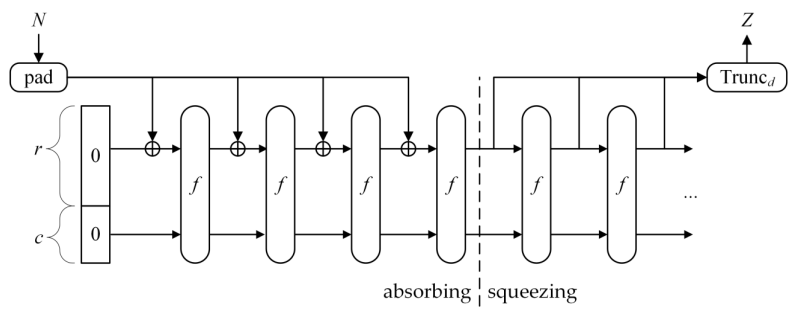
\includegraphics[width=0.7\linewidth]{sha3.png} \\ sponge-конструкция SHA-3}
    \end{figure}

    На схеме в качестве внутренней функции $f$ используется построенная функция $KECCAK$-$p[b, n_r](S)$.

    Итоговое преобразование, используемое в работе SHA-3 может быть записано в виде: \\ $KECCAK[c](N, d)$ = $SPONGE[KECCAK$-$p[1600, 24], pad10*1, 1600-c](N, d)$, где $pad10*1$ --- некоторая функция расширения входного сообщения.
    
\end{enumerate}


\subsection{ГОСТ Р 34.11-94}

Описание алгоритма ГОСТ Р 34.11-94 приводится в соответствии с описанием, приведенным в стандарте \cite{gost94}. На вход алгоритма поступает произвольное двоичное сообщение; на выходе алгоритм выдает 256-битный хеш входного сообщения. Приведем описание работы данного алгоритма:

\begin{enumerate}
    \item При подсчете хеш-значения используется специальная шаговая функция хеширования $\chi = \chi(M, H)$ (отображение, которое преобразует два 256-битных блока данных в один), алгоритм вычисления которой включает в себя три части: 
    \begin{enumerate}
        \item Генерация ключей --- 256-битных слов $K_1, K_2, K_3$ и $K_4$.

        Пусть $X = x_4 \mathbin\Vert x_3 \mathbin\Vert x_2 \mathbin\Vert x_1 = y_{32} \mathbin\Vert ... \mathbin\Vert y_1$ --- 256-битное слово, $x_1, x_2, x_3$ и $x_4$ --- 64-битные слова, образующие $X$, а $y_1, ..., y_{32}$ --- 8-битные слова, образующие $X$. Тогда определим преобразования $A(X) = (x_1 \oplus x_2) \mathbin\Vert x_4 \mathbin\Vert x_3 \mathbin\Vert x_2$ и $P(X) = y_{\phi(32)} \mathbin\Vert ... \mathbin\Vert y_{\phi(1)}$, где $\phi(i+1+4\cdot(k-1)) = 8\cdot i + k$, где $i = 0, ..., 3$; $k = 1, ..., 8$.

        Пусть на вход шаговой функции поступили 256-битные слова $H$ и $M$. Тогда для вычисления ключей будут выполнены следующие действия:

        \begin{itemize}
            \item $TEMP_1 = H$, $TEMP_2 = M$, $K_1 = P(TEMP_1 \oplus TEMP_2)$;
            \item Для $i=2, 3, 4$: $TEMP_1 = A(TEMP_1) \oplus C_i$, $TEMP_2 = A(A(TEMP_2))$, $K_i = P(TEMP_1 \oplus TEMP_2)$, где $C_2 = 0, C_3 = 0xff00ffff000000ffff0000ff00ffff0000ff00ff00ff00ffff00ff00ff00ff00, C_4 = 0$.
        \end{itemize}

        \item Шифрующее преобразование

        Пусть на вход шаговой функции поступили 256-битные слова $H$ и $M$. На данном этапе осуществляется зашифрование 64-битных подслов слова $H = h_4 \mathbin\Vert h_3 \mathbin\Vert h_2 \mathbin\Vert h_1$ на сгенерированных ключах $K_1, K_2, K_3$ и $K_4$.

        Шифрование происходит следующим образом: $s_i = E_{K_i}(h_i)$, где $i = 1, 2, 3, 4$, через $E_{K_i}$ обозначен алгоритм шифрования 64-битного блока на ключе $K_i$ по ГОСТ 28147 в режиме простой замены. В результате образуется 256-битное слово $S = s_4 \mathbin\Vert s_3 \mathbin\Vert s_2 \mathbin s_1$.

        \item Перемешивающее преобразование

        Определим функцию $\psi$, принимающую 256-битный блок $X = x_{16} \mathbin\Vert ... \mathbin\Vert x_1$ и возвращающую значение $\psi(X) = x_{1} \oplus x_2 \oplus x_3 \oplus x_4 \oplus x_{13} \oplus x_{16} \mathbin\Vert x_{16} \mathbin\Vert ... \mathbin\Vert x_2$.
        
    \end{enumerate}

    Таким образом, в качестве значения шаговой функции хеширования $\chi$, принимающей 256-битные блоки $M$ и $H$, определяется значение $\chi(M, H) = \psi^{61}(H \oplus \psi(M \oplus \psi^{12}(S)))$.

    \item Процедура вычисления хеш-функции сообщения $M = m_n \mathbin\Vert ... \mathbin\Vert m_1$, где $m_n, ..., m_1$ --- разбиение $M$ на 256-битные блоки (длина $m_n$ может быть менее 256 бит), с использованием шаговой функции хеширования состоит из следующих шагов:

    \begin{enumerate}
        \item Этап 1 --- инициализация

        \begin{itemize}
            \item $H = IV$, где $IV$ --- произвольный 256-битный блок, $H$ --- текущее значение хеш-функции;
            \item $\Sigma = 0^{256}$, где $\Sigma$ --- текущее значение контрольной суммы;
            \item $L = 0^{256}$, где $L$ --- длина сообщения.
        \end{itemize}

        \item Этап 2 --- циклическая обработка блоков $m_1, ..., m_{n-1}$; при обработке очередного блока $m_i$, $i = 1, ..., n-1$, выполняются следующие действия:

        \begin{itemize}
            \item $H = \chi(m_i, H)$;
            \item $L = L + 256$, где сложение 256-битных блоков происходит по модулю $2^{256}$;
            \item $\Sigma = \Sigma + m_i$, где сложение 256-битных блоков происходит по модулю $2^{256}$.
        \end{itemize}

        \item Этап 3 --- обработка финального блока $m_n$

        \begin{itemize}
            \item $L = L + |m_n|$;
            \item В начало блока $m_n$ дописываются незначащие нули, пока длина блока не станет равна 256;
            \item $\Sigma = \Sigma + m_n$, где сложение 256-битных блоков происходит по модулю $2^{256}$;
            \item $H = \chi(m_n, H)$;
            \item $H = \chi(L, H)$;
            \item $H = \chi(\Sigma, H)$.
        \end{itemize}
    \end{enumerate}
    Хеш-значением для входного сообщения $M$ является полученное на последнем шаге значение $H$.
\end{enumerate}

\subsection{ГОСТ 34.11-2018 (Стрибог)}

Описание алгоритма ГОСТ 34.11 - 2018 (Стрибог) приводится в соответствии с описанием, приведенным в стандарте \cite{gost2018}. На вход алгоритма поступает произвольное двоичное сообщение; на выходе алгоритм выдает 256-битный хеш входного сообщения или 512-битный хеш входного сообщения. Приведем описание работы данного алгоритма:


В работе алгоритма используются следующие константы, таблицы и функции:

\begin{enumerate}

    \item Векторы инициализации $IV$: для хеш-функции с длиной хеша в 512 бит $IV = 0^{512}$, для хеш-функции с длиной хеша в 256 бит $IV = (00000001)^{64}$;

    \item 512-битные шестнадцатеричные константы $C_1, ..., C_{12}$:

    \begin{itemize}
        \item $C_1 = b1085bda1ecadae9ebcb2f81c0657c1f2f6a76432e45d016714eb88d7585c4fc\\
        4b7се09192676901a2422a08a460d31505767436cc744d23dd806559f2a64507$;
        \item $C_2 = 6fa3b58aa99d2f1a4fe39d460f70b5d7f3feea720a232b9861d55e0f16b50131\\
        9ab5176b12d699585cb561c2db0aa7ca55dda21bd7cbcd56e679047021b19bb7$;
        \item $C_3 = f574dcac2bce2fc70a39fc286a3d843506f15e5f529c1f8bf2ea7514b1297b7b\\
        d3e20fe490359eb1c1c93a376062db09c2b6f443867adb31991e96f50aba0ab2$;
        \item $C_4 = ef1fdfb3e81566d2f948e1a05d71e4dd488e857e335c3c7d9d721cad685e353f\\
        a9d72c82ed03d675d8b71333935203be3453eaa193e837f1220cbebc84e3d12e$;
        \item $C_5 = 4bea6bacad4747999a3f410c6ca923637f151c1f1686104a359e35d7800fffbd\\
        bfcd1747253af5a3dfff00b723271a167a56a27ea9ea63f5601758fd7c6cfe57$;
        \item $C_6 = ae4faeae1d3ad3d96fa4c33b7a3039c02d66c4f95142a46c187f9ab49af08ec6\\
        cffaa6b71c9ab7b40af21f66c2bec6b6bf71c57236904f35fa68407a46647d6e$;
        \item $C_7 = f4c70e16eeaac5ec51ac86febf240954399ec6c7e6bf87c9d3473e33197a93c9\\
        0992abc52d822c3706476983284a05043517454ca23c4af38886564d3a14d493$;
        \item $C_8 = 9b1f5b424d93c9a703e7aa020c6e41414eb7f8719c36de1e89b4443b4ddbc49a\\
        f4892bcb929b069069d18d2bd1a5c42f36acc2355951a8d9a47f0dd4bf02e71e$;
        \item $C_9 = 378f5a541631229b944c9ad8ec165fde3a7d3a1b258942243cd955b7e00d0984\\
        800a440bdbb2ceb17b2b8a9aa6079c540e38dc92cb1f2a607261445183235adb$;
        \item $C_{10} = abbedea680056f52382ae548b2e4f3f38941e71cff8a78db1fffe18a1b336103\\
        9fe76702af69334b7a1e6c303b7652f43698fad1153bb6c374b4c7fb98459ced$;
        \item $C_{11} = 7bcd9ed0efc889fb3002c6cd635afe94d8fa6bbbebab07612001802114846679\\
        8a1d71efea48b9caefbacd1d7d476e98dea2594ac06fd85d6bcaa4cd81f32d1b$;
        \item $C_{12} = 378ee767f11631bad21380b00449b17acda43c32bcdf1d77f82012d430219f9b\\
        5d80ef9d1891cc86e71da4aa88e12852faf417d5d9b21b9948bc924af11bd720$.
    \end{itemize}

    \item Перестановка $\pi$ на множестве; $\{0, ..., 255 \}$ \begin{longtable}{|p{0.5cm}|p{0.5cm}|p{0.5cm}|p{0.5cm}|p{0.5cm}|p{0.5cm}|p{0.5cm}|p{0.5cm}|p{0.5cm}|p{0.5cm}|p{0.5cm}|p{0.5cm}|p{0.5cm}|p{0.5cm}|p{0.5cm}|p{0.5cm}|}
    \hline
    252 & 238 & 221 & 17 & 207 & 110 & 49 & 22 & 251 & 196 & 250 & 218 & 35 & 197 & 4 & 77 \\ 
    \hline
    233 & 119 & 240 & 219 & 147 & 46 & 15 & 186 & 23 & 54 & 241 & 187 & 20 & 205 & 95 & 193 \\
    \hline
    249 & 24 & 101 & 90 & 226 & 92 & 239 & 33 & 129 & 28 & 60 & 66 & 139 & 1 & 142 & 79 \\ 
    \hline
    5 & 132 & 2 & 174 & 227 & 106 & 143 & 160 & 6 & 11 & 237 & 152 & 127 & 212 & 211 & 31 \\
    \hline
    235 & 52 & 44 & 81 & 234 & 200 & 72 & 171 & 242 & 42 & 104 & 162 & 253 & 58 & 206 & 204 \\ 
    \hline
    181 & 112 & 14 & 86 & 8 & 12 & 118 & 18 & 191 & 114 & 19 & 71 & 156 & 183 & 93 & 135 \\
    \hline
    21 & 161 & 150 & 41 & 16 & 123 & 154 & 199 & 243 & 145 & 120 & 111 & 157 & 158 & 178 & 177 \\
    \hline
    50 & 117 & 25 & 61 & 255 & 53 & 138 & 126 & 109 & 84 & 198 & 128 & 195 & 189 & 13 & 87 \\
    \hline
    223 & 245 & 36 & 169 & 62 & 168 & 67 & 201 & 215 & 121 & 214 & 246 & 124 & 34 & 185 & 3 \\
    \hline
    224 & 15 & 236 & 222 & 122 & 148 & 176 & 188 & 220 & 232 & 40 & 80 & 78 & 51 & 10 & 74 \\
    \hline
    167 & 151 & 96 & 115 & 30 & 0 & 98 & 68 & 26 & 184 & 56 & 130 & 100 & 159 & 38 & 65 \\
    \hline
    173 & 69 & 70 & 146 & 39 & 94 & 85 & 47 & 140 & 163 & 165 & 125 & 105 & 213 & 149 & 59 \\
    \hline
    7 & 88 & 179 & 64 & 134 & 172 & 29 & 247 & 48 & 55 & 107 & 228 & 136 & 217 & 231 & 137 \\
    \hline
    225 & 27 & 131 & 73 & 76 & 63 & 248 & 254 & 141 & 83 & 170 & 144 & 202 & 216 & 133 & 97 \\
    \hline
    32 & 113 & 103 & 164 & 45 & 43 & 9 & 91 & 203 & 155 & 37 & 208 & 190 & 229 & 108 & 82 \\
    \hline
    89 & 166 & 116 & 210 & 230 & 244 & 180 & 192 & 209 & 102 & 175 & 194 & 57 & 75 & 99 & 182 \\
    \hline
    \caption{Таблица перестановки $\pi$}
    \end{longtable}

    \item Перестановка $\tau$ на множестве $\{0, ..., 63 \}$;
    
    \begin{longtable}{|p{0.5cm}|p{0.5cm}|p{0.5cm}|p{0.5cm}|p{0.5cm}|p{0.5cm}|p{0.5cm}|p{0.5cm}|p{0.5cm}|p{0.5cm}|p{0.5cm}|p{0.5cm}|p{0.5cm}|p{0.5cm}|p{0.5cm}|p{0.5cm}|}
    \hline
    0 & 8 & 16 & 24 & 32 & 40 & 48 & 56 & 1 & 9 & 17 & 25 & 33 & 41 & 49 & 57 \\
    \hline
    2 & 10 & 18 & 26 & 34 & 42 & 50 & 58 & 3 & 11 & 19 & 27 & 35 & 43 & 51 & 59 \\
    \hline
    4 & 12 & 20 & 28 & 36 & 44 & 52 & 60 & 5 & 13 & 21 & 29 & 37 & 45 & 53 & 61 \\ 
    \hline
    6 & 14 & 22 & 30 & 38 & 46 & 54 & 62 & 7 & 15 & 23 & 31 & 39 & 47 & 55 & 63 \\
    \hline
    \caption{Таблица перестановки $\tau$}
    
    \end{longtable}

    \item Преобразование $l$, принимающее на вход 64-битный блок данных и заключающееся в умножении справа данного блока на заданную матрицу $A$ над полем $GF(2)$. Строки матрицы $A$ определены в виде шестнадцатеричных констант следующим образом (увеличение номера строки слева направо, сверху вниз):

    \begin{figure}[h!]
    \center{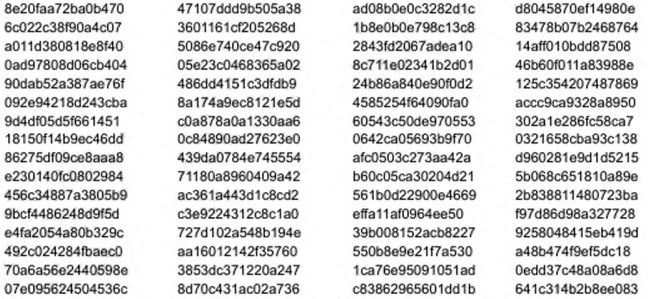
\includegraphics[width=0.7\linewidth]{gost.png} \\ Строки матрицы $A$}
    \end{figure}

    \item Функция $S = S(a)$, принимающая 512-битный блок $a = a_{63} \mathbin\Vert ... \mathbin\Vert a_0$, где $a_{63}, ..., a_0$ --- 8-битные блоки, и выдающая значение $S(a) = \pi(a_{63}) \mathbin\Vert ... \mathbin\Vert \pi(a_0)$;

    \item Функция $P = P(a)$, принимающая 512-битный блок $a = a_{63} \mathbin\Vert ... \mathbin\Vert a_0$, где $a_{63}, ..., a_0$ --- 8-битные блоки, и выдающая значение $P(a) = a_{\tau(63)} \mathbin\Vert ... \mathbin\Vert a_{\tau(0)}$;

    \item Функция $L = L(a)$, принимающая 512-битный блок $a = a_{7} \mathbin\Vert ... \mathbin\Vert a_0$, где $a_{7}, ..., a_0$ --- 64-битные блоки, и выдающая значение $L(a) = l(a_{7}) \mathbin\Vert ... \mathbin\Vert l(a_0)$;

    \item Значение хеш-функции сообщения вычисляется с использованием функции сжатия $g_N = g_N(h, m)$, где $h, m, N$ --- 512-битные блоки. Функция сжатия возвращает 512-битное значение $g_N(h, m)$, которое определяется следующим образом: $g_N(h, m) = E(LPS(h \oplus N), m) \oplus h \oplus m$, где функция $E = E(K, m) = K_{13} \oplus LPS(K_{12} \oplus ... LPS(K_2 \oplus LPS(m \oplus K_1))...)$, где через $LPS(x)$ обозначен результат последовательного применения функций $L, P, S$: $LPS(x) = L(P(S(x)))$, $K$ --- 512-битный блок.

    Значения $K_1, ..., K_{13}$ определяются следующим образом: $K_1 = K$, $K_i = LPS(K_{i-1} \oplus C_{i-1})$, $i = 2, ..., 13$.
    
\end{enumerate}

Процедура вычисления хеш-значения для произвольного сообщения $M = m_n \mathbin\Vert ... \mathbin\Vert m_1$, где $m_n, ..., m_1$ --- разбиение $M$ на 512-битные блоки (длина $m_n$ может быть мене 512 бит), состоит из следующих этапов:

\begin{enumerate}
    \item Этап 1 --- инициализация

    \begin{itemize}
        \item $h = IV$;
        \item $N = 0^{512}$;
        \item $\Sigma = 0^{512}$.
    \end{itemize}

    \item Этап 2 --- циклическая обработка блоков $m_1, ..., m_{n-1}$; при обработке очередного блока $m_i$, $i = 1, ..., n-1$, выполняются следующие действия:

    \begin{itemize}
        \item $h = g_N(h, m_i)$;
        \item $N = N + 512$, где сложение 512-битных блоков происходит по модулю $2^{512}$;
        \item $\Sigma = \Sigma + m_i$, где сложение 512-битных блоков происходит по модулю $2^{512}$.
    \end{itemize}


    \item Этап 3 --- обработка финального блока $m_n$

    \begin{itemize}
        \item В начало блока $m_n$ дописывается один единичный бит, после чего дописываются нулевые биты, пока длина блока не станет равна 512 (либо не дописываются, если длина уже равна 512);
        \item $h = g_N(h, m_n)$;
        \item $N = N + |m_n|$, где $|m_n|$ --- длина блока $m_n$ до начала его обработки, сложение происходит по модулю $2^{512}$;
        \item $\Sigma = \Sigma + m_n$, где сложение 512-битных блоков происходит по модулю $2^{512}$;
        \item $h = g_0(h, N)$;
        \item $H = g_0(h, \Sigma)$;
    \end{itemize}

    Если для сообщения $M$ необходимо выдать 512-битный хеш, то после всех проделанных операций будет возвращено вычисленное на последнем шаге алгоритма значение $H$; если необходимо выдать 256-битный хеш, то после всех проделанных операций будут возвращены старшие 256 бит вычисленного на последнем шаге алгоритма значения $H$.
    
\end{enumerate}


\subsection{BLAKE-256}

Описание алгоритма BLAKE-256 приводится на основе спецификации хеш-функции, представленной в \cite{blake}. На вход алгоритма поступает произвольное двоичное сообщение длины не более $2^{64} - 1$; на выходе алгоритм выдает 256-битный хеш входного сообщения. Приведем описание работы данного алгоритма: 

\begin{enumerate}
    \item Перед началом работы алгоритма определяются восемь шестнадцатеричных векторов инициализации, шестнадцать шестнадцатеричных констант и десять перестановок на множестве $\{ 0, ..., 15 \}$:

    \begin{longtable}{|p{2.6cm}|p{2.6cm}|p{2.6cm}|p{2.6cm}|}
\hline
$IV_0 = 6A09E667$ & $IV_1 = BB67AE85$ & $IV_2 = 3C6EF372$ & $IV3 = A54FF53A$ \\
\hline
$IV4 = 510E527F$ & $IV5 = 9B05688C$ & $IV6 = 1F83D9AB$ & $IV7 = 5BE0CD19$ \\
\hline
\caption{Таблица значений векторов инициализации $IV_0, ..., IV_{7}$}
\end{longtable}

\begin{longtable}{|p{2.6cm}|p{2.6cm}|p{2.6cm}|p{2.6cm}|}
\hline
$c_0 = 243F6A88$ & $c_1 = 85A308D3$ & $c_2 = 13198A2E$ & $c_3 = 03707344$ \\
\hline
$c_4 = A4093822$ & $c_5 = 299F31D0$ & $c_6 = 082EFA98$ & $c_7 = EC4E6C89$ \\
\hline
$c_8 = 452821E6$ & $c_9 = 38D01377$ & $c_{10} = BE5466CF$ & $c_{11} = 34E90C6C$ \\
\hline
$c_{12} = C0AC29B7$ & $c_{13} = C97C50DD$ & $c_{14} = 3F84D5B5$ & $c_{15} = B5470917$ \\
\hline
\caption{Таблица значений констант $c_0, ..., c_{15}$}
\end{longtable}

\begin{longtable}{|p{0.5cm} | p{4.5cm}|}
\hline
$\sigma_0$ & 0 1 2 3 4 5 6 7 8 9 10 11 12 13 14 15 \\
\hline
$\sigma_1$ & 14 10 4 8 9 15 13 6 1 12 0 2 11 7 5 3 \\
\hline
$\sigma_2$ & 11 8 12 0 5 2 15 13 10 14 3 6 7 1 9 4  \\
\hline
$\sigma_3$ & 7 9 3 1 13 12 11 14 2 6 5 10 4 0 15 8 \\
\hline
$\sigma_4$ & 9 0 5 7 2 4 10 15 14 1 11 12 6 8 3 13 \\
\hline
$\sigma_5$ & 2 12 6 10 0 11 8 3 4 13 7 5 15 14 1 9 \\
\hline
$\sigma_6$ & 12 5 1 15 14 13 4 10 0 7 6 3 9 2 8 11 \\
\hline
$\sigma_7$ & 13 11 7 14 12 1 3 9 5 0 15 4 8 6 2 10 \\
\hline
$\sigma_8$ & 6 15 14 9 11 3 0 8 12 2 13 7 1 4 10 5 \\
\hline
$\sigma_9$ & 10 2 8 4 7 6 1 5 15 11 9 14 3 12 13 0 \\
\hline
\caption{Перестановки $\sigma_0, ..., \sigma_{9}$}
\end{longtable}

    \item Работа алгоритма основана на функции сжатия $compress = compress(h, m, s, t)$, которая принимает 256-битное значение $h = h_0 \mathbin\Vert h_7$, 512-битное значение $m = m_0 \mathbin\Vert ... \mathbin\Vert m_{15}$, 128-битное значение $s = s_0 \mathbin\Vert ... \mathbin\Vert s_3$ и 64-битное значение $t = t_0 \mathbin\Vert t_1$, где все промежуточные блоки состоят из 32 бит. Данная функция возвращает 256-битное значение $h^{'} = h_0^{'} \mathbin\Vert ... \mathbin\Vert h_7^{'}$.

    \item При вычислении значения функции $compress$ используется набор из 16 слов $v_0, ..., v_{15}$, совокупность которых называется состоянием. Инициализация состояния происходит следующим образом:

    \begin{longtable}{|p{2.6cm}|p{2.6cm}|p{2.6cm}|p{2.6cm}|}
\hline
$v_0 = h_0$ & $v_1 = h_1$ & $v_2 = h_2$ & $v_3 = h_3$ \\
\hline
$v_4 = h_4$ & $v_5 = h_5$ & $v_6 = h_6$ & $v_7 = h_7$ \\
\hline
$v_8 = s_0 \oplus c_0$ & $v_9 = s_1 \oplus c_1$ & $v_{10} = s_2 \oplus c_2$ & $v_{11} = s_3 \oplus c_3$ \\
\hline
$v_{12} = t_0 \oplus c_4$ & $v_{13} = t_0 \oplus c_5$ & $v_{14} = t_1 \oplus c_6$ & $v_{15} = t_1 \oplus c_7$ \\
\hline
\caption{Инициализация $v_0, ..., v_{15}$}
\end{longtable}

\item Операции над состоянием $v_0, ..., v_{15}$ производятся посредством серии обращений к раундовой функции $G_i(a, b, c, d)$. После инициализации состояния запускается серия из четырнадцати раундов, каждый из которых состоит из следующих обращений:

\begin{longtable}{|p{2.6cm}|p{2.6cm}|p{2.6cm}|p{2.6cm}|}
\hline
$G_0(v_0, v_4, v_8, v_{12})$ & $G_1(v_1, v_5, v_9, v_{13})$ & $G_2(v_2, v_6, v_{10}, v_{14})$ & $G_3(v_3, v_7, v_{11}, v_{15})$ \\
\hline
$G_4(v_0, v_5, v_{10}, v_{15})$ & $G_5(v_1, v_6, v_{11}, v_{12})$ & $G_6(v_2, v_7, v_8, v_{13})$ & $G_7(v_3, v_4, v_9, v_{14})$ \\
\hline
\caption{Операции в раунде}
\end{longtable}

Во время раунда $0 \leq r \leq 13$ функцией $G_i(a, b, c, d)$ выполняются следующие действия:

\begin{enumerate}
    \item $a = a + b + (m_{\sigma_{r \mod 10}(2i)} \oplus c_{\sigma_{r \mod 10}(2i+1)})$;
    \item $d = (d \oplus a) >>> 16$;
    \item $c = c + d$;
    \item $b = (b \oplus c) >>> 12$;
    \item $a = a + b + (m_{\sigma_{r \mod 10}(2i+1)} \oplus c_{\sigma_{r \mod 10}(2i)})$;
    \item $d = (d \oplus a) >>> 8$;
    \item $c = c + d$;
    \item $b = (b \oplus c) >>> 7$.
\end{enumerate}

После выполнения всех раундов происходят следующие операции, в результате которых определяется выход функции $compress$:

\begin{itemize}
    \item $h_0^{'} = h_0 \oplus s_0 \oplus v_0 \oplus v_8$;
    \item $h_1^{'} = h_1 \oplus s_1 \oplus v_1 \oplus v_9$;
    \item $h_2^{'} = h_2 \oplus s_2 \oplus v_2 \oplus v_{10}$;
    \item $h_3^{'} = h_3 \oplus s_3 \oplus v_3 \oplus v_{11}$;
    \item $h_4^{'} = h_4 \oplus s_0 \oplus v_4 \oplus v_{12}$;
    \item $h_5^{'} = h_5 \oplus s_1 \oplus v_5 \oplus v_{13}$;
    \item $h_6^{'} = h_6 \oplus s_2 \oplus v_6 \oplus v_{14}$;
    \item $h_7^{'} = h_7 \oplus s_3 \oplus v_7 \oplus v_{15}$.
\end{itemize}

\item Хеширование входного сообщения $m$ выполняется следующим образом:

\begin{enumerate}
    \item Сообщение расширяется путем добавления битов по следующему правилу:

    \begin{enumerate}
        \item В конец сообщения приписывается один единичный бит;
        \item В конец сообщения приписываются нулевые биты до тех пор, пока длина сообщения не станет сравнима с 447 по модулю 512;
        \item В конец сообщения приписывается еще один единичный бит;
        \item В конец сообщения приписывается 64-битное представление длины сообщения $L$.
    \end{enumerate}
    После данных преобразований длина сообщения оказывается кратной 512.

    \item Входное сообщение $m$ делится на 512-битные блоки $m = m_0 \mathbin\Vert ... \mathbin\Vert m_{N-1}$. Для каждого блока вычисляется его длина $L_i$, $0 \leq i \leq N-1$, исключая при подсчете те биты, которые были добавлены на предыдущем шаге.

    \item Пользователем определяется значение 128-битной соли $s = s_0 \mathbin\Vert ... \mathbin\Vert s_3$.

    \item Выполняется присваивание $h^0 = IV_0 \mathbin\Vert ... \mathbin\Vert IV_7$.

    \item В цикле выполняется вызов функции сжатия: $h^{i+1} = compress(h^i, m^i, s, L^i)$, $0 \leq i \leq N-1$.
    
\end{enumerate}
    В качестве хеш-значения входного сообщения выдается посчитанное на последней итерации значение $h^N$.
\end{enumerate}

\subsection{RIPEMD-256}

\subsubsection{Описание хеш-функции}

Описание алгоритма RIPEMD-256 приводится на основе работ \cite{ripemd1} и \cite{ripemd2} разработчиков данной хеш-функции. На вход алгоритма поступает произвольное двоичное сообщение; на выходе алгоритм выдает 256-битный хеш входного сообщения. Опишем работу данного алгоритма:


В работе алгоритма используются следующие функции, константы и таблицы:
\begin{enumerate}
    \item Четыре параметрические функции:

    \begin{itemize}
        \item $f(j, x, y, z) = x \oplus y \oplus z$, где $0 \leq j \leq 15$;
        \item $f(j, x, y, z) = (x \wedge y) \vee (\bar x \wedge z)$, где $16 \leq j \leq 31$;
        \item $f(j, x, y, z) = (x \vee \bar y) \oplus z$, где $32 \leq j \leq 47$;
        \item $f(j, x, y, z) = (x \wedge z) \vee (y \wedge \bar z)$, где $48 \leq j \leq 63$.
    \end{itemize}

    \item Шестнадцатеричные константы:

    \begin{itemize}
        \item $K(j) = 0x00000000$, где $0 \leq j \leq 15$;
        \item $K(j) = 0x5A827999$, где $16 \leq j \leq 31$;
        \item $K(j) = 0x6ED9EBA1$, где $32 \leq j \leq 47$;
        \item $K(j) = 0x8F1BBCDC$, где $48 \leq j \leq 63$;
        \item $K^{'}(j) = 0x50A28BE6$, где $0 \leq j \leq 15$;
        \item $K^{'}(j) = 0x5C4DD124$, где $16 \leq j \leq 31$;
        \item $K^{'}(j) = 0x6D703EF3$, где $32 \leq j \leq 47$;
        \item $K^{'}(j) = 0x00000000$, где $48 \leq j \leq 63$.
    \end{itemize}

    \item Начальные значения:

    \begin{itemize}
        \item $h_0 = 0x67452301$; 
        \item $h_1 = 0xEFCDAB89$; 
        \item $h_2 = 0x98BADCFE$; 
        \item $h_3 = 0x10325476$;
        \item $h_4 = 0x76543210$;
        \item $h_5 = 0xFEDCBA98$; 
        \item $h_6 = 0x89ABCDEF$;
        \item $h_7 = 0x01234567$.
    \end{itemize}

    \item Таблицы $s = s_i$ и $s^{'} = s^{'}_i$, $0 \leq i \leq 63$, определяющие величину выполняемого циклического сдвига (изменение индекса слева направо, сверху вниз):

    \begin{longtable}{|p{6cm}|}
\hline
11, 14, 15, 12, 5, 8, 7, 9, 11, 13, 14, 15, 6, 7, 9, 8 \\
\hline
7, 6, 8, 13, 11, 9, 7, 15, 7, 12, 15, 9, 11, 7, 13, 12 \\
\hline
11, 13, 6, 7, 14, 9, 13, 15, 14, 8, 13, 6, 5, 12, 7, 5 \\
\hline
11, 12, 14, 15, 14, 15, 9, 8, 9, 14, 5, 6, 8, 6, 5, 12 \\
\hline
\caption{Таблица $s$}
\end{longtable}

    \begin{longtable}{|p{6cm}|}
\hline
8, 9, 9, 11, 13, 15, 15, 5, 7, 7, 8, 11, 14, 14, 12, 6 \\
\hline
9, 13, 15, 7, 12, 8, 9, 11, 7, 7, 12, 7, 6, 15, 13, 11 \\
\hline
9, 7, 15, 11, 8, 6, 6, 14, 12, 13, 5, 14, 13, 13, 7, 5 \\
\hline
15, 5, 8, 11, 14, 14, 6, 14, 6, 9, 12, 9, 12, 5, 15, 8 \\
\hline
\caption{Таблица $s^{'}$}
\end{longtable}

    \item Таблицы $r = r_i$ и $r^{'} = r^{'}_i$, $0 \leq i \leq 63$, определяющие ... (изменение индекса слева направо, сверху вниз):

    \begin{longtable}{|p{6cm}|}
\hline
0, 1, 2, 3, 4, 5, 6, 7, 8, 9, 10, 11, 12, 13, 14, 15 \\
\hline
7, 4, 13, 1, 10, 6, 15, 3, 12, 0, 9, 5, 2, 14, 11, 8 \\
\hline
3, 10, 14, 4, 9, 15, 8, 1, 2, 7, 0, 6, 13, 11, 5, 12 \\
\hline
1, 9, 11, 10, 0, 8, 12, 4, 13, 3, 7, 15, 14, 5, 6, 2 \\
\hline
\caption{Таблица $r$}
\end{longtable}

    \begin{longtable}{|p{6cm}|}
\hline
5, 14, 7, 0, 9, 2, 11, 4, 13, 6, 15, 8, 1, 10, 3, 12 \\
\hline
6, 11, 3, 7, 0, 13, 5, 10, 14, 15, 8, 12, 4, 9, 1, 2 \\
\hline
15, 5, 1, 3, 7, 14, 6, 9, 11, 8, 12, 2, 10, 0, 4, 13 \\
\hline
8, 6, 4, 1, 3, 11, 15, 0, 5, 12, 2, 13, 9, 7, 10, 14 \\
\hline
\caption{Таблица $r^{'}$}
\end{longtable}
\end{enumerate}

Перед началом вычисления хеш-значения сообщение расширяется путем добавления битов по следующему правилу:

\begin{enumerate}
    \item В конец сообщения приписывается один единичный бит;
    \item В конец сообщения приписываются нулевые биты до тех пор, пока длина сообщения не станет сравнима с 448 по модулю 512;
    \item В конец сообщения приписывается 64-битное представление длины сообщения (если исходная длина сообщения превышает $2^{64}$, то от ее битовой длины используется только младшие 64 бит).
\end{enumerate}
После данных преобразований длина сообщения оказывается кратной 512.

После описанных преобразований расширенное входное сообщение $X$ разделяется на $t$ 256-битных блоков: $X = X[0] \mathbin\Vert ... \mathbin\Vert X[t-1]$. Каждый блок $X[i]$ при этом подразбивается на 16 32-битных блоков: $X[i] = X[i][0] \mathbin\Vert ... \mathbin\Vert X[i][15]$, $0 \leq i \leq i-1$. Алгоритм вычисления хеш-значения (сложения производятся по модулю $2^{32}$):

$For$ $i$ $=$ $0$ $to$ $t - 1$ $do$ \{ 

    \hspace{0.5cm} $A = h_0$; $B = h_1$; $C = h_2$; $D = h_3$;
    
    \hspace{0.5cm} $A^{'} = h_4$; $B^{'} = h_5$; $C^{'} = h_6$; $D^{'} = h_7$;

    \hspace{0.5cm} $For$ $j$ $=$ $0$ $to$ $63$ $do$ \{

    \hspace{1cm} $TEMP = (A + f(j, B, C, D) + X[i][r_j] + K(j)) <<< s_j$;

    \hspace{1cm} $A = D$; $D = C$; $C = B$; $B = TEMP$;

    \hspace{1cm} $TEMP = (A + f(63 - j, B^{'}, C^{'}, D^{'}) + X[i][r^{'}_j] + K^{'}(j)) <<< s_j^{'}$;

    \hspace{1cm} $A^{'} = D^{'}$; $D^{'} = C^{'}$; $C^{'} = B^{'}$; $B^{'} = TEMP$;

    \hspace{1cm} Если $j = 15$, то значения $A$ и $A^{'}$ меняются местами;

    \hspace{1cm} Если $j = 31$, то значения $B$ и $B^{'}$ меняются местами;

    \hspace{1cm} Если $j = 47$, то значения $C$ и $C^{'}$ меняются местами;

    \hspace{1cm} Если $j = 63$, то значения $D$ и $D^{'}$ меняются местами;

    \hspace{0.5cm} \}

    \hspace{0.5cm} $h_0 = h_0 + A$; $h_1 = h_1 + B$; $h_2 = h_2 + C$; $h_3 = h_3 + D$;

    \hspace{0.5cm} $h_4 = h_4 + A^{'}$; $h_5 = h_5 + B^{'}$; $h_6 = h_6 + C^{'}$; $h_7 = h_7 + D^{'}$; 
    
\}

Итоговым хеш-значением для входного сообщения является полученное после последней итерации 256-битное значение $h_0 \mathbin\Vert ... \mathbin\Vert h_7$.

\subsubsection{Анализ хеш-функции}

Хеш-функция RIPEMD-256 является расширением хеш-функции RIPEMD-128, которая выдает хеш-значение длиной в 128 бит. RIPEMD-256 предназначена для применения в приложениях, которым требуется более длинное значение хеш-функции без необходимости более высокого уровня безопасности, чем обеспечиваемый RIPEMD-128 (хотя удвоение хеш-значения и уменьшает вероятность коллизий). Хеш-функция RIPEMD-256 сконструирована на основе RIPEMD-128 путем инициализации двух параллельных потоков вычисления с разными начальными значениями и исключения комбинации двух потоков после последнего шага преобразования обновления состояния. Кроме того, после каждого раунда между двумя параллельными потоками вычислений происходит обмен некоторыми внутренними переменными состояния, чтобы сделать два потока зависимыми друг от друга.

Так как хеш-функция RIPEMD-256 не является более криптостойкой по сравнению с RIPEMD-128, и так как работ по анализу RIPEMD-256 в литературе практически не представлено, то далее будут описаны теоретические атаки, применимые к RIPEMD-128. Стоит также отметить, что эксплуатируемых на практике уязвимостей данного алгоритма на текущий момент не обнаружено.

В работе \cite{ripemdat1} была представлена атака на 38-раундовый RIPEMD-128, в результате которой со сложностью $2^{14}$ для хеш-функции была найдена коллизия. Предлагаемая авторами статьи стратегия поиска коллизии состоит из трех шагов:

\begin{enumerate}
    \item Поиск стартовой точки --- нахождение такой стартовой настройки
    (различия только в нескольких конкретных словах сообщений), которая с высокой вероятностью может привести к дифференциальной характеристике после 15 шага.

    Поскольку RIPEMD-128 имеет два потока с разной перестановкой слов сообщения, первым шагом в атаке является определение тех слов сообщения, которые могут содержать различия, учитывая несколько ограничений, позволяющих эффективно провести всю атаку в целом. 
    Прежде всего, авторы стремятся к получению дифференциальных характеристик с высокой вероятностью после 15 шага в обоих потоках (линиях) вычислений. Такие дифференциальные характеристики с высокой вероятностью могут быть построены, если различия, вносимые словами сообщения, немедленно устраняются с помощью локальных коллизий, охватывающих всего несколько шагов. Авторы делают акцент на рассмотрении двух слов сообщения: $m_0$ и $m_6$ ($M = m_0 \mathbin\Vert ... \mathbin\Vert m_{15}$), за счет чего объединением в одной линии двух локальных коллизий (что приводит к одной длительной локальной коллизии между этапами 3 и 20) удается к третьему раунду коллизию для 38 шагов RIPEMD-128.

    \begin{figure}[h!]
        \center{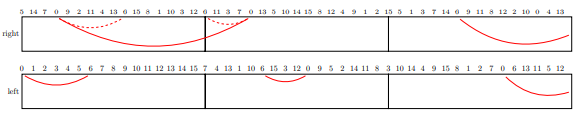
\includegraphics[width=0.6\linewidth]{ripemd1.png} \\ Локальные коллизии при использовании слов $m_0$ и $m_6$}
        \end{figure}
    
    \item Поиск дифференциальной характеристики

    После того, как была определена стартовая точка (то есть слова сообщения, которые могут содержать различия), авторы предлагают использовать автоматизированный инструмент для поиска дифференциальной характеристик с высокой вероятностью. Автоматическое устройство поиска основано на подходе, описанном в работе \cite{ripemdat3}, для поиска сложных нелинейных дифференциальных характеристик и подтверждающих пар сообщений для SHA-2. Основная идея заключается в рассмотрении дифференциальных характеристик, накладывающих произвольные условия на пары битов с использованием так называемых обобщенных условий. Обобщенные условия основаны на различиях в знаках битов и учитывают все 16 возможных условий для пар битов. Автоматическое устройство позволяет находить сложные нелинейные дифференциальные характеристики и решать нелинейные уравнения, включающие условия на слова состояния и свободные биты сообщения, то есть находить подтверждающие пары сообщений. Стоит отметить, что разница в сообщении не фиксируется до начала поиска, чтобы инструмент мог найти оптимальное решение. Сначала поиск происходит в первой линии --- с учетом наличия 14 ограничений на возможные значения участвующих в цепочке значений сложность поиска составляет примерно $2^{14}$. Аналогичный поиск происходит и во второй линии. 
    
    \item Поиск пары сообщений

    Чтобы выполнить все условия, налагаемые дифференциальной характеристикой в первом раунде, необходимо применить методы модификации сообщений. Авторы также с использованием автоматизированного инструмента добиваются модификации сообщения на первых 16 шагах. Также сложность модификации сообщения может быть компенсирована путем рандомизации, например, слова сообщения $m_{12}$, чтобы найти решение также для характеристики с высокой вероятностью во втором раунде (и в третьем раунде). Авторы отмечают, что на практике, используя приблизительно $2^{30}$ возможных значений для $m_{12}$, можно найти решение для дифференциальной характеристики (сложность $2^{14}$ после первого раунда), включая изменение сообщения, менее чем за секунду.
    
\end{enumerate}

Таким образом, со сложностью $2^{14}$ была построена коллизия для 38-шаговой хеш-функции RIPEMD-128.

\begin{figure}[h!]
        \center{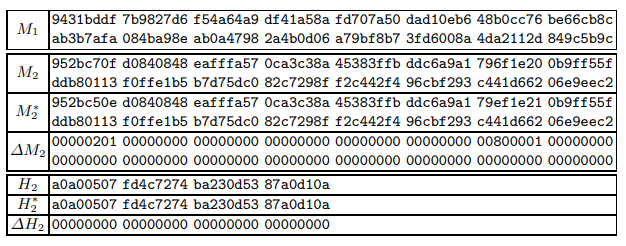
\includegraphics[width=0.6\linewidth]{ripemd2.png} \\ Построенная коллизия $M_2$ и $M_2^*$}
        \end{figure}

В статье \cite{ripemdat2} представлена атака на 40-раундовый RIPEMD-128, в результате которой со сложность $2^{35}$ для хеш-функции была найдена коллизия. Коллизия достигается путем построения 512-битных блоков $N \mathbin\Vert M$ и $N \mathbin\Vert M'$, где $N, M, M'$ --- 256-битные блоки. В статье предложен следующий алгоритм поиска коллизии состоит из следующих шагов:

Вычисления в RIPEMD-128 (как и в RIPEMD-256) происходят параллельно в рамках двух линий, условно обозначаемых как $line_1$ и $line_2$ (в описании алгоритма RIPEMD-256 это результаты первого в цикле циклического сдвига и второго соответственно).

\begin{enumerate}
    \item Авторы выбирают различия в сообщениях следующим образом: пусть $M = m_0 \mathbin\Vert ... \mathbin\Vert m_{15}$; $\Delta M = M' - M$ выбирается так, чтобы $\Delta m_i = 0$, $0 \leq i \leq 15, i \neq 2, i \neq 12$; $\Delta m_2 = 2^8$, $\Delta m_{12} = -2$. На основе данных условий определяются дифференциальные характеристики для $line_1$ и $line_2$. Выбор обоснован тем, что он приводит к возникновению локальной коллизии с 25 шага по 29 шага в операциях $line_1$ и локальной коллизии между 6 и 32 шагами в операциях $line_2$. Это свойство делает возможность проведения коллизионной атаки на 40-шаговый RIPEMD-128, используя различия в сообщениях, удовлетворяющих указанным свойствам.

    \item Авторами выводятся наборы достаточных условий, которые обеспечивают выполнение дифференциальных характеристик. Для данных условий устанавливается, что вероятность их выполнения приблизительно равна $2^{-35}$.

    \item Алгоритм поиска коллизий состоит из следующих шагов:

    \begin{enumerate}
        \item Необходимо случайно выбрать блоки $m_i$, $0 \leq i \leq 15$, $i \neq 12$, после чего их необходимо модифицировать так, чтобы был выполнен набор достаточных условий $line_1$, а также чтобы набор достаточных условий $line_2$ выполнялся с вероятностью $2^{-35}$;
        \item Если достаточные условия $line_2$ оказались не выполнены, то необходимо перейти к шагу а);
        \item Необходимо случайно выбрать блок $m_{12}$ и посчитать хеш-значения получившихся $M$ и $M'$ 40-шаговым RIPEMD-128. Если значения совпали, то выдать $M$ и $M'$. Иначе необходимо перейти к шагу а).
    \end{enumerate}
    
\end{enumerate}

Таким образом, с временной сложностью примерно $2^{35} + 2^{41}$ удается осуществить коллизионную атаку на 40-шаговую вариацию хеш-функции RIPEMD-128. Пример построения коллизии (для данных сообщений $\Delta m_2 = 2^8$, $\Delta m_{12} = -2$):
\begin{figure}[h!]
        \center{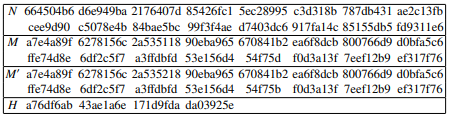
\includegraphics[width=0.6\linewidth]{attack2.png} \\ Построенная коллизия $N\mathbin\Vert M$ и $N\mathbin\Vert M'$}
        \end{figure}

\subsection{Whirlpool}

Описание хеш-функции Whirlpool приводится на основе статьи \cite{Whirlpool} разработчиков данной хеш-функции. На вход хеш-функции подается произвольное двоичное сообщение длины не более $2^{256} - 1$ бит; на выходе функция выдает 512-битный хеш входного сообщения. Опишем работу данного алгоритма:

Хеш-функция основана на специальном блочном шифре, который работает с 512-битными данными. Промежуточный результат вычисления хеш-значения называется состоянием, которое представляется квадратной матрицей состояния из восьми строк и восьми столбцов из элементов поля $GF(2^8)$. Пространство таких матриц будем далее обозначать через $M_{8x8}[GF(2^8)]$.

\begin{itemize}

    \item Преобразование $\mu$, преобразующее 512-битные блоки в обозначенные матрицы. Пусть $a \in GF(2^8)^{64}$, $b \in M_{8x8}[GF(2^8)]$. Тогда $\mu(a) = b \iff b_{i, j} = a_{8i + j}$, $0 \leq i, j \leq 7$.

    \item Преобразование $\gamma$. Пусть $a, b \in  M_{8x8}[GF(2^8)]$. Тогда $\gamma(a) = b \iff b_{i, j} = S[a_{i, j}]$, $0 \leq i, j \leq 7$.
    
    \begin{figure}[h!]
        \center{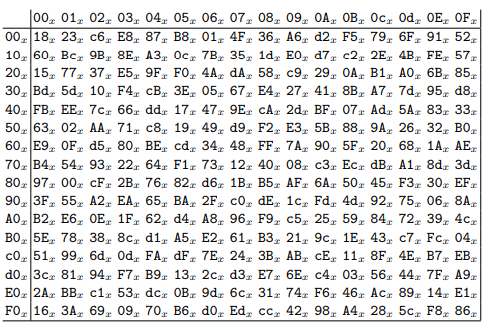
\includegraphics[width=0.6\linewidth]{whirlpool.png} \\ Таблица преобразования $S$}
        \end{figure}

    \item Преобразование $\pi$. Пусть $a, b \in  M_{8x8}[GF(2^8)]$. Тогда $\pi(a) = b \iff b_{i,j} = a_{(i-j) \mod 8, j}$, $0 \leq i, j \leq 7$.

    \item Преобразование $\theta$. Пусть $a, b \in  M_{8x8}[GF(2^8)]$. Тогда $\theta(a) = b \iff b = a \cdot C$.
    
    \begin{figure}[h!]
        \center{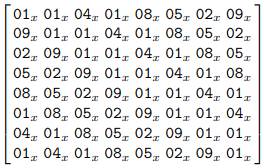
\includegraphics[width=0.5\linewidth]{whirlpool2.png} \\ Матрица $C$}
        \end{figure}

    \item Преобразование $\sigma[k]$. Пусть $a, b, k \in  M_{8x8}[GF(2^8)]$. Тогда $\sigma[k](a) = b \iff b_{i, j} = a_{i, j} \oplus k_{i, j}$, $0 \leq i, j \leq 7$.

    \item Раундовые константы $c^r$. Пусть $c^r \in  M_{8x8}[GF(2^8)]$, $r > 0$ --- номер раунда. Тогда:
    \begin{itemize}
        \item $c_{0, j}^r = S[8(r - 1) + j]$, $0 \leq j \leq 7$;
        \item $c_{i, j}^r = 0$, $1 \leq i \leq 7$, $0 \leq j \leq 7$.
    \end{itemize}

    \item Раундовая функция $\rho[k]$. Пусть $a, b, k \in  M_{8x8}[GF(2^8)]$. Тогда для каждого раунда $r$ раундовая функция имеет вид: $\rho[k](a) \equiv \sigma[k](\theta(\pi(\gamma(a))))$.

    \item Процедура расширения ключа. 512-битный ключ $K \in  M_{8x8}[GF(2^8)]$ расширяется до последовательности раундовых ключей $K^0, ..., K^R$ следующим образом:

    \begin{itemize}
        \item $K^0 = K$;
        \item $K^r = \rho[c^r](K^{r-1})$, $r > 0$.
    \end{itemize}

    Как правило, число раундов $R$ по умолчанию равно 10.

    \item Внутренний блочный шифр $W[K]$. Пусть $a, b, K \in  M_{8x8}[GF(2^8)]$. Тогда шифром выполняется следующая последовательность преобразований: $W[K](a) = \rho[K^r](\rho[K^{r-1}](...\rho[K^1](\sigma[K^0](a))...))$.
    
\end{itemize}

Процедура подсчета хеш-значения:
\begin{enumerate}
    \item К концу сообщения $M$ дописывается единичный бит;
    \item К концу сообщения $M$ дописываются нулевые биты, чтобы длина полученного сообщения была кратная 256 нечетное число раз;
    \item К концу сообщения $M$ дописывается 256-битное значение длины сообщения.
    \item Обработка сообщения:

    \begin{enumerate}
        \item Дополненное сообщение разбивается на 512-битные блоки $m_t \mathbin\Vert ... \mathbin\Vert m_1$.
        \item $\eta_i = \mu(m_i)$;
        \item $H_0 = \mu(IV)$, где $IV = 0^{512}$;
        \item $H_i = W[H_{i-1}](\eta_i) \oplus H_{i-1} \oplus \eta_i$, $1 \leq i \leq t$.
    \end{enumerate}
    
\end{enumerate}

В качестве хеш-значение сообщения $M$ возвращается значение $\mu^{-1}(H_t)$.

\subsection{Fast Syndrome Based Hash (FSB)}

Описание хеш-функции Fast Syndrome Based Hash приводится в соответствии с работой \cite{fsb} разработчиков данной хеш-функции. 

Алгоритм FSB основан на использовании структуры Меркла—Дамгарда, использует для вычисления функции сжатия случайную двоичную матрицу $H$ и имеет несколько параметров:

\begin{itemize}
    \item $n$ --- число столбцов матрицы $H$;
    \item $r$ --- число строк матрицы $H$ и число бит на выходе хеш-функции;
    \item $w$ --- число столбцов матрицы $H$, выбираемых из матрицы при подсчете значения функции сжатия;
    \item $s$ --- число бит на входе функции сжатия;
\end{itemize}
Для данных параметров должны выполняться условия: $s > r$, $s = w\log_2(\frac{n}{w})$.


Под словом веса $w$ и длины $n$ будем понимать $n$-битный блок данных, в котором содержится ровно $w$ единичных бит. Слово веса $w$ и длины $n$ является регулярным, если в каждом интервале от $(i-1)\frac{n}{w}$ до $i\frac{n}{w}$ содержится ровно один ненулевой элемент, $1 \leq i \leq w$.

Алгоритм вычисления функции сжатия следующий:

\begin{enumerate}
    \item Матрица $H$ разделятся на $w$ подматриц из $r$ строк и $\frac{n}{w}$ столбцов;
    \item Входное сообщение из $s$ бит разделяется на части $s_1, ..., s_w$ длины $\log_2(\frac{n}{w})$;
    \item Каждое значение $s_1, ..., s_w$ преобразуется в целое десятичное число от 1 до $\frac{n}{w}$;
    \item Для каждого значения $i$ из подматрицы $H_i$ выбирается соответствующий десятичному значению $s_i$ столбец;
    \item Выбранные $w$ столбцов побитово складываются, в результате чего образуется выход функции сжатия длины $r$.
    
\end{enumerate}

\section{Заключение}

В работе были описаны основные архитектуры построения хеш-функций: Sponge-конструкция и конструкция HAIFA, а также были рассмотрены хеш-функции MD5, SHA-1, SHA-256, SHA-3, ГОСТ Р 34.11-94, ГОСТ 34.11-2018 (Стрибог), BLAKE-256, RIPEMD-256, Whirlpool и Fast Syndrome Based Hash (FSB), построенные в том числе на основе указанных ранее конструкций. Также более подробно была рассмотрена хеш-функция RIPEMD-256. Данная хеш-функция является модернизацией хеш-функции RIPEMD-128 и предназначена для применения в приложениях, которым требуется более длинное значение хеш-значения без необходимости более высокого уровня безопасности, чем обеспечиваемый RIPEMD-128. Уязвимостей для алгоритма RIPEMD-256 на текущий момент не обнаружено. Вместе с тем известны теоретические атаки на ограниченные по раундам версии алгоритма RIPEMD-128, позволяющие совершить на алгоритм коллизионную атаку, что теоретически (в силу определенной преемственности алгоритмов) может быть перенесено на алгоритм RIPEMD-256. Также стоит отметить, что RIPEMD-256, очевидно, за счет увеличения длины хеш-значения теоретически является более стойким к коллизионной атаке, чем RIPEMD-128. Таким образом, лучшей атакой на RIPEMD-256 на текущей момент является атака путем полного перебора.
\end{document}